\documentclass{article}

%%%%%%%%%%%%%%%%%%%%%%%%%%%%%%%%%%%%%%%%%%%%%%%%%%%%%%%%%%%%%%%%%
%%%%%%%%%%%%%%%%%%%%%%%%%%%%%%%%%%%%%%%%%%%%%%%%%%%%%%%%%%%%%%%%%
% JENGA diagrams adapted from cube eg in
%   http://www.texample.net/tikz/examples/plane-partition/

\usepackage{tikz}
\usetikzlibrary{patterns}
\usepackage{ifthen}

\newcommand\xaxis{210}
\newcommand\yaxis{-30}
\newcommand\zaxis{ 90}

\newcommand\jengaOddtopside[3]{
  \fill[fill=yellow, draw=black,
        shift={(\xaxis:#1)},shift={(\yaxis:#2)},shift={(\zaxis:#3)}]
        (0,0) -- (30:3) -- (1.73205,2) -- (150:1) --(0,0);
}

\newcommand\jengaOddleftside[3]{
  \fill[preaction={fill, red}, pattern=dots, draw=black,
        shift={(\xaxis:#1)},shift={(\yaxis:#2)},shift={(\zaxis:#3)}]
        (0,0) -- (0,-1) -- (210:1) --(150:1)--(0,0);
}

\newcommand\jengaOddrightside[3]{
  \fill[fill=blue, draw=black,
        shift={(\xaxis:#1)},shift={(\yaxis:#2)}, shift={(\zaxis:#3)}]
        (0,0) -- (30:3) -- (2.59807,0.5) --(0,-1)--(0,0);
}

\newcommand\jengaOddLevel[3]{
  \jengaOddtopside{#1}{#2}{#3}
  \jengaOddleftside{#1}{#2}{#3}
  \jengaOddrightside{#1}{#2}{#3}
}

\newcommand\jengaEventopside[3]{
  \fill[fill=yellow, draw=black,
        shift={(\xaxis:#1)},shift={(\yaxis:#2)},shift={(\zaxis:#3)}]
        (0,0) -- (30:1) -- (-1.73205,2) -- (-2.59807,1.5) -- (0,0);
}

\newcommand\jengaEvenleftside[3]{
  \fill[fill=red, draw=black,
        shift={(\xaxis:#1)},shift={(\yaxis:#2)},shift={(\zaxis:#3)}]
        (0,0) -- (0,-1) -- (-2.59807,0.5) -- (-2.59807,1.5) --(0,0);
}

\newcommand\jengaEvenrightside[3]{
  \fill[preaction={fill, blue}, pattern=dots, draw=black,
        shift={(\xaxis:#1)},shift={(\yaxis:#2)},shift={(\zaxis:#3)}]
        (0,0) -- (30:1) -- (-30:1) --(0,-1)--(0,0);
}

\newcommand\jengaEvenLevel[3]{
  \jengaEventopside{#1}{#2}{#3}
  \jengaEvenleftside{#1}{#2}{#3}
  \jengaEvenrightside{#1}{#2}{#3}
}

\newcounter{height}
\newcounter{count}
\newcounter{parity}

\newcommand\jengaTower[1]{
  \setcounter{height}{-1}
  \setcounter{parity}{0}
  \foreach \level in {#1} {
    \addtocounter{height}{1}
    \setcounter{count}{-1}
    \foreach \piece in \level {
      \addtocounter{count}{1}
      \ifthenelse{ \piece = 1 } {
         \ifthenelse{ \value{parity} = 0  }
            { \jengaEvenLevel{\value{count}}{2}{\value{height}} }
            { \jengaOddLevel{2}{\value{count}}{\value{height}} }
      }
      {}
    }
    \ifthenelse{ \value{parity} = 0 }
      {\setcounter{parity}{1}}
      {\setcounter{parity}{0}}
  }
}
%%%%%%%%%%%%%%%%%%%%%%%%%%%%%%%%%%%%%%%%%%%%%%%%%%%%%%%%%%%%%%%%%
%%%%%%%%%%%%%%%%%%%%%%%%%%%%%%%%%%%%%%%%%%%%%%%%%%%%%%%%%%%%%%%%%

\begin{document}

\title{Macro for {\sc jenga} diagrams}
\maketitle

Jenga latex macro was adapted from cube eg in 

  http://www.texample.net/tikz/examples/plane-partition/

Check tex file for the implementation.

Using the Jenga macro as

\begin{verbatim}
  \jengaTower{{1,0,1},{1,0,1},{0,1,1},{1,1,1},{1,1,0},{0,1,1}}
  \jengaTower{{1,0,1},{1,0,1},{0,1,1},{1,1,1},{1,1,1},{0,1,1}}
  \jengaTower{{0,1,0},{1,0,1},{0,1,1},{1,1,1},{1,1,1},{0,1,1}}
\end{verbatim}

produces:

\begin{center}
  \resizebox{4cm}{4cm}{
    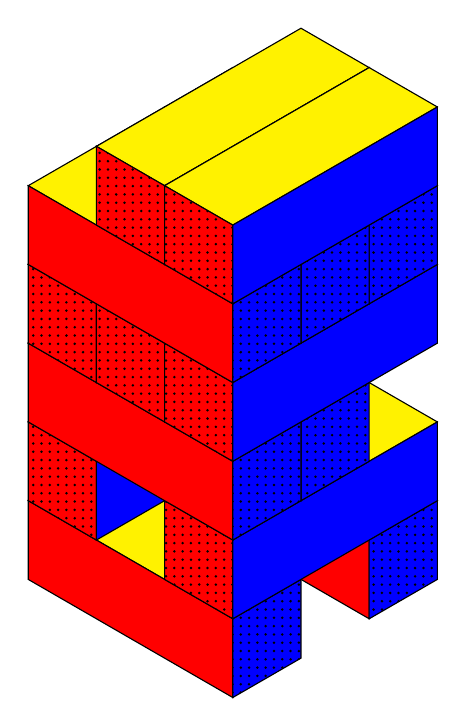
\begin{tikzpicture}
      \jengaTower{{1,0,1},{1,0,1},{0,1,1},{1,1,1},{1,1,1},{0,1,1}}
    \end{tikzpicture}
  }
\end{center}

\begin{center}
  \resizebox{4cm}{4cm}{
    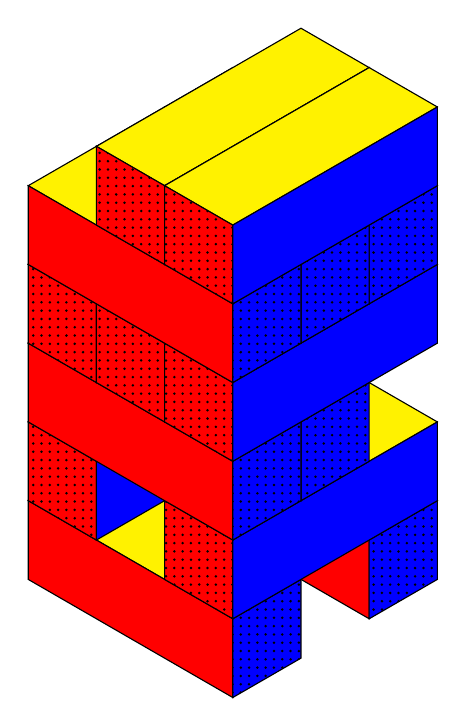
\begin{tikzpicture}
      \jengaTower{{1,0,1},{1,0,1},{0,1,1},{1,1,1},{1,1,1},{0,1,1}}
    \end{tikzpicture}
  } \quad
  \resizebox{4cm}{4cm}{
    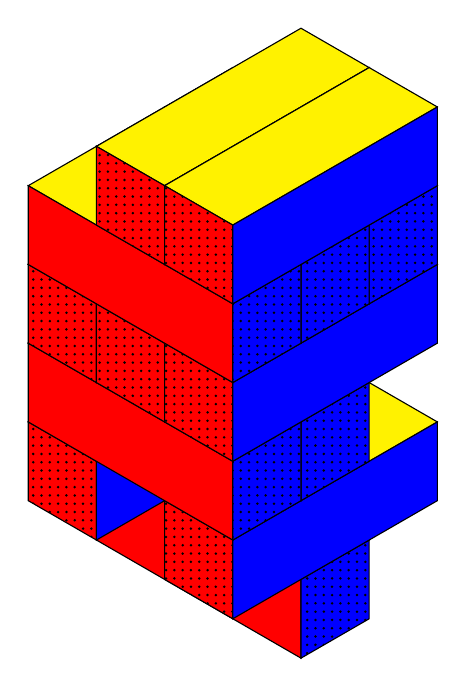
\begin{tikzpicture}
      \jengaTower{{0,1,0},{1,0,1},{0,1,1},{1,1,1},{1,1,1},{0,1,1}}
    \end{tikzpicture}
  }
\end{center}

%%%%%%%%%%%%%%%%%%%%%%%%%%%%%%%%%%%%%%%%%%
% to draw a complete Jenga Tower:

% \begin{center}
%   \resizebox{3cm}{6cm}{
%     \begin{tikzpicture}
%   \jengaTower{{1,1,1},{1,1,1},{1,1,1},{1,1,1},{1,1,1},{1,1,1},{1,1,1},{1,1,1},{1,1,1},{1,1,1},{1,1,1},{1,1,1},{1,1,1},{1,1,1},{1,1,1},{1,1,1},{1,1,1},{1,1,1}}
%     \end{tikzpicture}
%   }
% \end{center}
%%%%%%%%%%%%%%%%%%%%%%%%%%%%%%%%%%%%%%%%%%

\end{document}




